%
% direction.tex
%
\renewcommand{\thisname}{Chart::Direction}
\section{\thisname}
\name{\thisname}
\file{Direction.pm}
\requires{Chart::Base, GD, Carp, FileHandle}
\begin{Description}
The class \thisclass creates a diagram based on polar
coordinates. This type of diagram is occasionally referred to as a
\emph{radial} or as a \emph{radar} chart. \thisclass plots data
specified by angle (\eg, wind direction) and absolute value (\eg, wind
strength). The first dataset to add is always the set of angles in
degrees. The second set contains the absolute values. How additional
datasets should be entered depends on the option \attruse{pairs} (cf.
below). By default, \thisclass will draw a point chart. You can also
get a lines chart by setting the option \attruse{point} to
\literal{false} and the option \attruse{line} to \literal{true}. If you
want a lines and point chart, then set both \attruse{point} and
\attruse{line} to \literal{true}. In addition, \thisclass plots arrows
from the center to the point or to the end of the line if the option
\attruse{arrow} is set to \literal{true}. \thisclass is a subclass of
\class{Chart::Base}.
\end{Description}

\example
\begin{figure}[ht]
  \begin{center}
    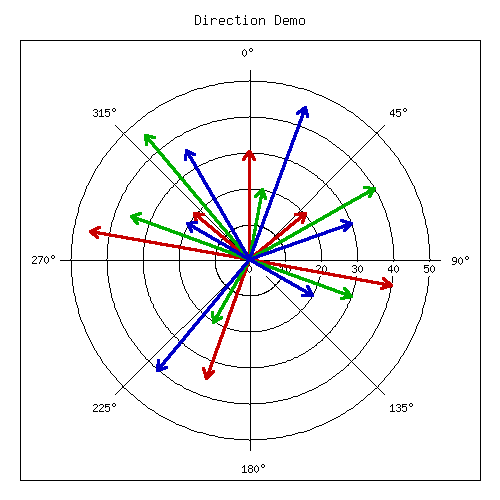
\includegraphics[width = 8cm, height =8cm]{direction.png}
  \end{center}
  \caption{Direction chart}
  \label{fig:direction}
\end{figure}
\begin{verbatim}
use Chart::Direction;
$g = Chart::Direction->new(500,500);

$g->add_dataset( 0, 100, 50, 200, 280, 310);
$g->add_dataset(30,  40, 20,  35,  45,  20);

$g->add_dataset(10, 110, 60, 210, 290, 320);
$g->add_dataset(20,  30, 40,  20,  35,  45);

$g->add_dataset(20, 120, 70, 220, 300, 330);
$g->add_dataset(45,  20, 30,  40,  20,  35,);

%hash = ( 'title'           => 'Direction Demo',
          'angle_interval'  => 45,
          'precision'       => 0,
          'arrow'           => 'true',
          'point'           => 'false',
          'include_zero'    => 'true',
          'pairs'           => 'true',
          'legend'          => 'none',
          'grey_background' => 'false'
        );

$g->set(%hash);

$g->png("direction.png");
\end{verbatim}

\constructorblurb{\thisname}

\begin{AttrDecl}{angle\_interval}
This option tells \thisclass how many angle lines should be drawn. It is
the difference between two angle lines. The default value is 30, which
means that one line will be drawn every 30 degrees. Not all values are
permissible; the valid ones are: 0, 5, 10, 15, 20, 30, 45, and 90. If
you choose 0, \thisclass will draw no lines.
\end{AttrDecl}

\begin{AttrDecl}{arrow}
Draws an arrow from the center of the chart to the point if set to
\literal{true}. By default \literal{false}.
\end{AttrDecl}

\begin{AttrDecl}{brush\_size}
Sets the width of the lines in pixels. Default is 6.
\end{AttrDecl}

\begin{AttrDecl}{line}
Connects the points with lines if set to \literal{true}. Defaults to
\literal{false}.
\end{AttrDecl}

\begin{AttrDecl}{max\_circles}
Sets the maximum number of circles to draw when generating the set of
circles. Default is 100. This limit is used to avoid plotting an
unreasonably large number of circles if non-round values are used for
\attruse{min\_val} and \attruse{max\_val}. The value for
\attruse{max\_circles} should be at least 5 times that of
\attruse{min\_circles}.
\end{AttrDecl}

\begin{AttrDecl}{min\_circles}
Sets the minimum number of circles to draw when generating a scale.
Default is 4, minimum is 2.
\end{AttrDecl}

\begin{AttrDecl}{pairs}
This option tells \thisclass how to handle additional datasets. If
\attruse{pairs} is set to \literal{true}, \thisclass uses the first
dataset as a set of degrees and the second dataset as a set of values.
Then, the third set is a set of degrees and the fourth a set of values,
and so forth. If \attruse{pairs} is set to \literal{false}, \thisclass
uses the first dataset as a set of angles and all following datasets as
sets of values. Defaults to \literal{false}.
\end{AttrDecl}

\begin{AttrDecl}{point}
Indicates to draw points for representing the data values. Possible
values: \literal{true} and \literal{false}, by default \literal{true}.
\end{AttrDecl}

\begin{AttrDecl}{pt\_size}
Sets the radius of the points in pixels. Default is 18.
\end{AttrDecl}

\begin{AttrDecl}{sort}
Sorts the data in ascending order if set to \literal{true}. Should be
set if the input data is not sorted and \attruse{line} is set to
\literal{true}. Defaults to \literal{false}.
\end{AttrDecl}
